\documentclass[tikz]{standalone}
\begin{document}
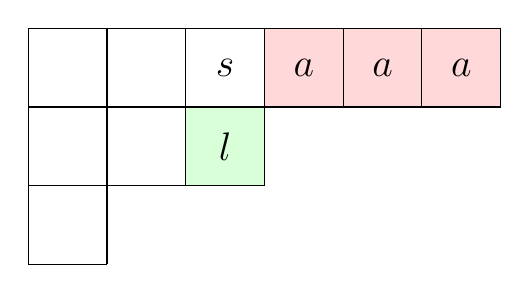
\begin{tikzpicture}
\filldraw[red!15] (3,0) rectangle (6,-1);\filldraw[green!15] (2,-1) rectangle (3,-2);
\draw (0,0) -- (6,0);\draw (0,-1) -- (6,-1);\draw (0,-2) -- (3,-2);\draw (0,-3) -- (1,-3);\draw (1,0) -- (1,-3);\draw (2,0) -- (2,-2);\draw (3,0) -- (3,-2);\draw (4,0) -- (4,-1);\draw (5,0) -- (5,-1);\draw (6,0) -- (6,-1);\draw (0,0) -- (0,-3);
\begin{scope}[font=\Large]
  \draw (2.5, -0.5) node{$s$};\draw (3.5, -0.5) node{$a$};\draw (4.5, -0.5) node{$a$};\draw (5.5, -0.5) node{$a$};\draw (2.5, -1.5) node{$l$};
\end{scope}
\end{tikzpicture}
\end{document}
